\documentclass[12pt]{article}
\usepackage[english]{babel}
\usepackage{subcaption}
\usepackage{float}
\usepackage{natbib}
\usepackage{url}
\usepackage[utf8x]{inputenc}
\usepackage{amsmath}
\usepackage{graphicx}
\graphicspath{{images/}}
\usepackage{parskip}
\usepackage{fancyhdr}
\usepackage{vmargin}
\usepackage{hyperref}
\usepackage{listings}
\usepackage{color} %red, green, blue, yellow, cyan, magenta, black, white
\definecolor{mygreen}{RGB}{28,172,0} % color values Red, Green, Blue
\definecolor{mylilas}{RGB}{170,55,241}


\setmarginsrb{3 cm}{2.5 cm}{3 cm}{2.5 cm}{1 cm}{1.5 cm}{1 cm}{1.5 cm}
\usepackage{listings}
\title{Final Project}
\author{Akwasi A. Obeng}                    
\date{December 08, 2019}										
\makeatletter
\let\thetitle\@title
\let\theauthor\@author
\let\thedate\@date
\makeatother

\pagestyle{fancy}
\fancyhf{}
\rhead{\theauthor}
\lhead{\thetitle}
\cfoot{\thepage}

\begin{document}

%%%%%%%%%%%%%%%%%%%%%%%%%%%%%%%%%%%%%%%%%%%%%%%%%%%%%%%%%%%%%%%%%%%%%%%%%%%%%%%%%%%%%%%%%

\lstset{language=Matlab,%
    %basicstyle=\color{red},
    breaklines=true,%
    morekeywords={matlab2tikz},
    keywordstyle=\color{blue},%
    morekeywords=[2]{1}, keywordstyle=[2]{\color{black}},
    identifierstyle=\color{black},%
    stringstyle=\color{mylilas},
    commentstyle=\color{mygreen},%
    showstringspaces=false,%without this there will be a symbol in the places where there is a space
    numbers=left,%
    numberstyle={\tiny \color{black}},% size of the numbers
    numbersep=9pt, % this defines how far the numbers are from the text
    emph=[1]{for,end,break},emphstyle=[1]\color{red}, %some words to emphasise
    %emph=[2]{word1,word2}, emphstyle=[2]{style},    
  }


\begin{titlepage}
	\centering
    \vspace*{0.5 cm}
    
\includegraphics[scale = 0.1]{uon.jpeg}\\[1.0 cm]	% University Logo
    \textsc{\LARGE Drone Navigation with Reinforcement Learning}\\[2.0 cm]	% University Name
	\textsc{\Large Formal Report}\\[0.5 cm]				% Course Code
	\textsc{\large Project}\\[0.5 cm]				% Course Name
	\rule{\linewidth}{0.2 mm} \\[0.4 cm]
	{ \huge \bfseries \thetitle}\\
	\rule{\linewidth}{0.2 mm} \\[1.5 cm]
	
	\begin{minipage}{0.4\textwidth}
		\begin{flushleft} \large
			\emph{Author:}\\
			\theauthor
			\end{flushleft}
			\end{minipage}~
			\begin{minipage}{0.4\textwidth}
			\begin{flushright} \large
			\emph{DirectoryID:} \\
			obenga01 
		\end{flushright}
	\end{minipage}\\[2 cm]
	
	{\large \thedate}\\[2 cm]
 
	\vfill
	
\end{titlepage}

%%%%%%%%%%%%%%%%%%%%%%%%%%%%%%%%%%%%%%%%%%%%%%%%%%%%%%%%%%%%%%%%%%%%%%%%%%%%%%%%%%%%%%%%%

\tableofcontents
\pagebreak

\section{Abstract}
In recent times, the increase in the usage of automobiles has caused difficulty in transporting goods between two places.
As a result, the alternative use of employing aerial robots such as drones in transporting goods has gained a lot of popularity
due to the reduced traffic and the effiency and ease of transporting goods from one place to another. 
However, aerial robots face the disadvantage of navigating dynamic obstacles  and being able to interact with the environment in an intelligent 
manner. Due to these difficulties, it is imperative that the drone be equipped with some form amount of intelligence. This paper focuses on how
reinforcement learning can be applied to enable the drone navigate its environment intelligently and efficiently.

\section{Introduction}
Drones in recent times are being used for surveillance in military and for transportation purposes. Amazon currently is trying to commercialize
the use of drones for transporting products from one place to another. The problem of operating a drone is that even if a drone has been 
programmed to follow a specified path using the most intelligent of algorithms, there are bound to be uncertainties. How well the drone responds 
to such situations is of paramount importance as it could mean a drone accidentaly hitting an obstacle, or detecting unreasonable things or
venturing into really dangerous and costly situations.

\begin{figure}[h]
    \centering
    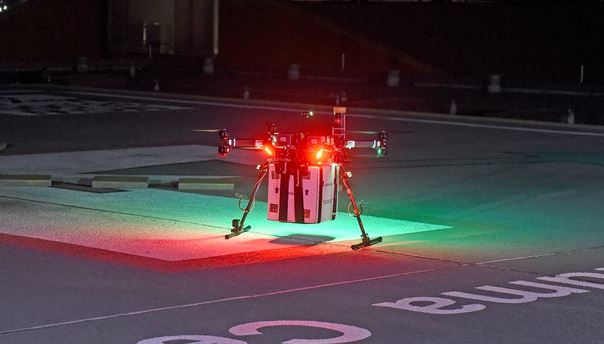
\includegraphics[width=7cm]{kidney}
    \caption{Drone delivering kidney}
    \label{fig:Drone delivering kidney}
\end{figure}
This paper focuses on the first phase of the project which is training a drone to interact with its environment in an intelligent way devoid of 
any sensing capability. Suitable reinforcement learning algorithms are tried and tested to see how well the drone learns- that is, how much reward
can be accumulated from experience. 

\section{Reinforcement Learning Introduction}
Reinforcement learning algorithms differ from the traditional machine learning algorithms, supervised and unsupervised learning, in the sense 
that, the agent interacts with the environment and continous  to learn from experience. Unlike supervised learning, where there is a target 
that is to be matched, in reinforcement Learning, the exact target or goal may not be known fully. 
The agent continuous to change its behavior in response
to the amount of reward received for a particular action. RL also differs from unspervised learning because the goal is not just to  find 
structure or similarity in the data, but rather actions or behaviors that maximize the reward in the short term or long term depending on the
problem at hand.
 
\section{Problem Description}
The goal of the project is for the drone to navigate through the gateways as illustrated in the figure shown below. The rewards have been placed
right in the middle of the gateways and the drone is supposed to orient and learn to generate a path that accumulates the most reward.


\begin{figure}[h]
    \centering
    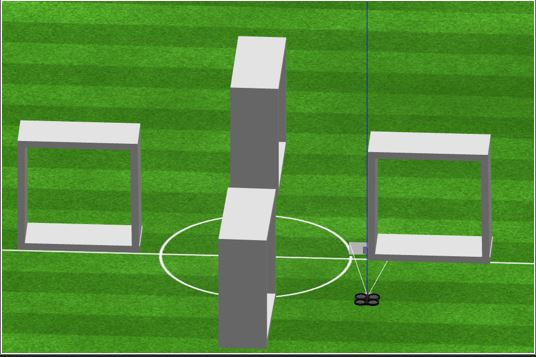
\includegraphics[width=8cm]{gazebo}
    \caption{World created in ROS}
    \label{fig:3D environment created in matplotlib}
\end{figure}

\subsection{Problem Characteristics}
\begin{itemize} 
  \item \textbf{State Space} -  Continuous State space $\rightarrow$ (Position p,Orientation o) 
  \item \textbf{Action Space} - left, right,up,down, forward 
  \item \textbf{Environment} - We focus on \textbf{static environment} for now.
\end{itemize}


\subsection{Gazebo Parameters}
Due to the huge workspace field, the robot is confined to a rectangular workspace with the dimensions given below.
\begin{align}
  min_x&: -2.7  \quad \nonumber
max_x: 7 \\                     
  min_y&: -2.5  \quad  \nonumber
max_y: 7.3 \\                   
  min_z&: 0.00  \quad \nonumber
max_z: 3.00
\end{align}
NB. Gazebo uses SI units. Therefore distances are in meters.


\section{Approach}
Both qlearning and deep qlearning where tested to see how well the drone learned. A brief summary and results using both approaches 
is given below.
\subsection{Reward Structure}
\begin{table}[h]
  \centering
\begin{tabular}{ |p{3cm}||p{3cm}|p{3cm}|p{3cm}|  }
 \hline
 \multicolumn{2}{|c|}{Reward structure} \\
 \hline
 Reward     & Values\\
 \hline
 forward   & 1\\
 turn&   1.5\\
 up&1\\
 down&1.5\\
 goal& 2000  \\
 \hline
\end{tabular}
\end{table}

The drone gets a goal reward of 300, each time it passes through any of the centers of the gateways 
\textbf{(-1.6,2.2,2.0),(2.33,-1.14,2.0),( 5.7,2.29,2.0),(2.0,6.1,2.0)} at some thresholded radius of 0.7m. 
To prevent the drone from circling about the same 
center in a gateway, the \textbf{goal reward} is set to \textbf{zero} after center has been reached and reset back to \textbf{300} after any of the other centers other than the previous one has been reached.

\subsection{Qlearning}
 Q learning tries to maximize the action-value  using the update rule given below.

\begin{equation}
  Q(S_t,A_t) \leftarrow Q(S_t,A_t) + \alpha[R_{t+1}+\gamma \max\limits_a Q(S_{t+1},a)- Q(S_t,A_t)]
\end{equation}
where, 
\begin{align}
  \alpha &\rightarrow  \text{learning rate}, \text{A measure of movement for every time step}     \nonumber  \\
  \gamma &\rightarrow  \text{Discount factor}, \text{A measure of  future or immediate rewards}  \nonumber \\
  A      &\rightarrow \text{Action}  \nonumber \\
  S      &\rightarrow \text{State} \nonumber
\end{align}

Qlearning works with discrete state and action spaces. To apply qlearning to our problem, we discretize the continous state space 
apply the update rule shown above.

\subsubsection{Hyperparameters}
\begin{itemize}
  \item \textbf{alpha}: 0.01 - Small learning rate to ensure convergence
  \item \textbf{gamma}: 0.6 - Fairly big discount factor as the drone can easily recover from bad orientations. 
    No need for heavy dependence on future rewards.
  \item \textbf{epsilon}: 0.995 - More exploration in the beginning  
  \item \textbf{epsilon\_discount}: 0.998  - Exploration should last for several episodes. Need 1000 episodes to reach an epsilon value 
    of about 0.1
\end{itemize}

\subsubsection{Policy, Steps  And Episodes}
Qlearning was applied to the problem and the drone was trained using \textbf{epsilon-greedy policy} for about \textbf{1000 episodes} and 
\textbf{700 steps}.

\subsubsection{Qlearning Results}
\begin{figure}[h]
    \centering
    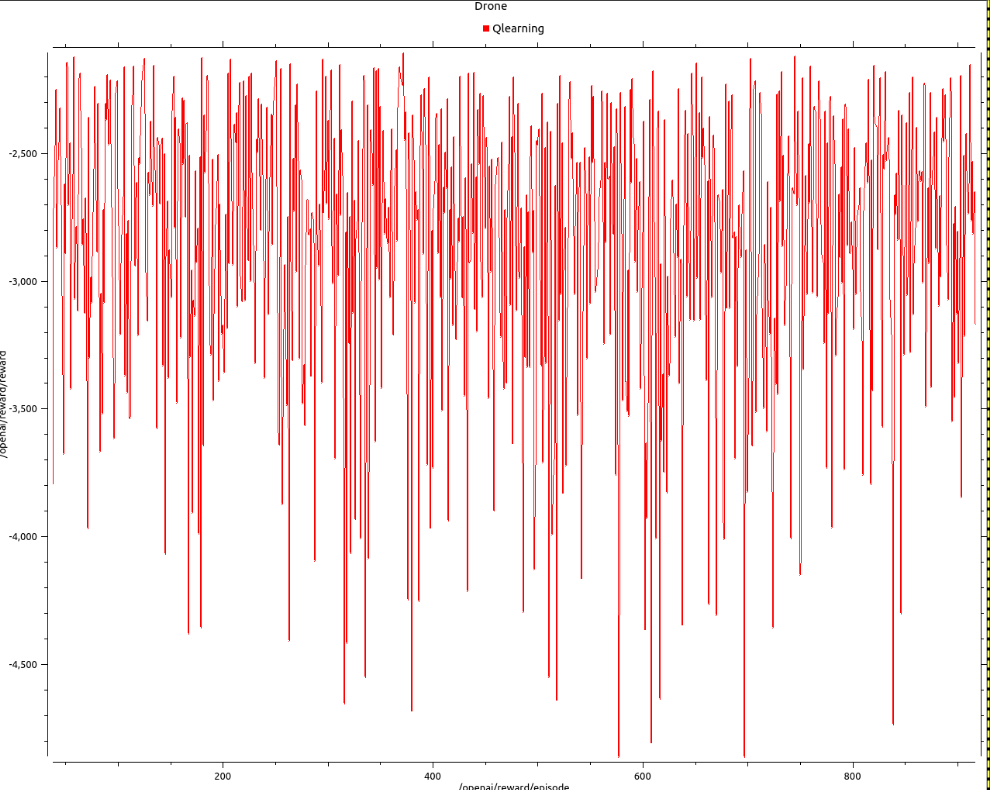
\includegraphics[width=12cm]{qlearn}
    \caption{Qlearning Results}
    \label{fig:3D environment created in matplotlib}
\end{figure}

Clearly, it can be seen from the graph that, the robot is not maximizing the amount reward that can be generated because, the state space is
huge. Even after 1000 episodes, the drone is nowhere close to desired optimal solution.  For qlearning to work, the resolution of the 
discretization can be increased-this results in huge state space- and the number of episodes can be increased. Better results can be achieved
but the downside is that it would take a lot of time and space to achieve the desired result

\subsubsection{limitations}
\textbf{Qlearning} is not an appropriate solution as:
\begin{itemize}
  \item \textbf{State space is huge(continuous state space)}- The drone can be in particular position with some orientation. 
  \item \textbf{Slow to learn} - Qlearning tries to learn the value of each state space. This is not ideal as state space
        close(suitable metric) together coudld have yield similar values. Therefore, a method which approximates the value function
        using a suitable function is more desirable.
  \item \textbf{Huge memory} - Qlearning learning requires a lot of memory space for this problem
\end{itemize}

\subsection{Deep Qlearning}
\subsubsection{Function Approximation}
Instead of storing all the possible states with their associated action-values, the values corresponding to the states are approximated. 
States that are really close together may tend to have the same values,or even yet, there may be an underlying structure or pattern to 
action-values associated to the different states. Therefore a Deep Network, is employed to approximate these values. 
to the states.

The goal then is to find parameters w, that minimizes the distance(suitable metric) between the actual value function $v_\pi(s)$ and 
the approximate value function $\bar{v}(s,w)$.
The cost function then becomes,
\begin{equation}
    J(w) =  E_\pi[(v_\pi(S) - \bar{v}(S,w))^2]
\end{equation}

Unlike in Supervised learning, 
where the target(actual value)  is known, the actual value function($v_\pi$) is not known and continuous to 
change.  The update rule for action-value associated with a state is therefore given as

\begin{equation}
  \Delta w = \alpha(q_\pi(S,A)-\bar{q}(S,A,w))\nabla_{w}\bar{q}(S,A,w)
\end{equation}

\subsubsection{Mini Batch Training Method}
Mini batch update,with a \textbf{batch size of 100},  was used as the ordinary batch update is too slow and incremental changes using
the stochastic update is susceptible to noise as it doesn't capture the pattern really well. In every iteration, 100 points(S,A,R,S') are 
sampled and used in updating the weights.


\subsubsection{Architecture} 
The network was trained with two hidden units. The properties are tabulated below. The values were attained through trial and error.

\begin{table}[h]
  \centering
\begin{tabular}{ |p{3cm}||p{3cm}|p{3cm}|p{3cm}|  }
 \hline
 \multicolumn{3}{|c|}{Network Architecture} \\
 \hline
 Layers     & Units & Activation Function \\
 \hline
 Input layer  & state space dim & $-$ \\
 First layer  & 60 & relu \\
 Second layer & 75 & relu \\
 Output layer & action space dim & linear \\
 \hline
 \multicolumn{3}{|c|}{Other Properties} \\
 \hline
 Optimization Method &Adam & $-$ \\
 \hline
 loss Function &MSE &$-$ \\
 \hline
\end{tabular}
\end{table}


\newpage
\subsubsection{Policy, Steps and Episodes}
Qlearning was applied to the problem and the drone was trained using \textbf{epsilon-greedy policy} for about \textbf{6000 episodes} and 
\textbf{3000 steps}.
\subsubsection{Hyperparameters}
\begin{itemize}
  \item \textbf{alpha}: 0.01 - Small learning rate to ensure convergence
  \item \textbf{gamma}: 0.6 - Fairly big discount factor as the drone can easily recover from bad orientations. 
    No need for heavy dependence on future rewards.
  \item \textbf{epsilon}: 0.995 - More exploration in the beginning  
  \item \textbf{epsilon\_discount}: 0.998  - Exploration should last for several episodes. Need 1000 episodes to reach an epsilon value 
    of about 0.1
\end{itemize}
\subsection{Results}
\begin{figure}[h]
    \centering
    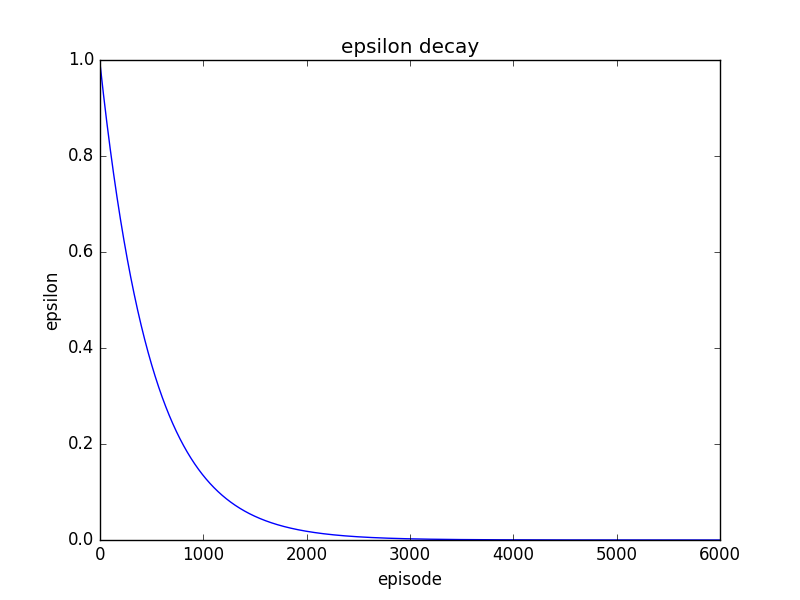
\includegraphics[width=10cm]{epsilon_decay}
    \caption{epsilon decay}
    \label{fig:3D environment created in matplotlib}
\end{figure}

\subsection{Tools Used}
\begin{itemize}
  \item ROS -Kinetic
  \item Gazebo 
  \item Openai-gym - The robot was trained using openai library
  \item Openai-ros - Openai ros makes interfacing robots in ros with easy. Refer to ros wiki for tutorials. 
  \item Deep Neural Network - The code utilized keras which utilized tensor flow backend and starter deep qlearning code 
    from \href{https://github.com/keon/deep-q-learning/blob/master/dqn.py}{Keon-Deep Qlearning}
\end{itemize}
\section{Analysis}
\section{Conclusions}
Clearly, it can be noted that, deep qlearning outperforms qlearning when the state space is big and continuous. Qlearning is much more useful
when both action space and state space are discrete and small. Depending on the type of problem, we can switch to different types of learning
methods. For Example, if the drone is constrained to move in a plane with some predefined number of steps, then qlearning will be more suitable.

\section{Future Work}
We plan to continue working on the problem trying out different reinforcement learning architectures. From there, we incorporate 
dynamic obstacles and include sensing capability of the drone in the learning process- that is, camera and lidar. Then we create a suitable
environment with a slightly more complex goal and examine how well the drone learns.
\section{Bibliography}
https://github.com/keon/deep-q-learning/blob/master/dqn.py \\
https://www.theconstructsim.com/how-to-launch-drone-simulation-locally/ \\
https://www.theconstructsim.com/using-openai-ros/
http://wiki.ros.org/openai\_ros

\section{Appendix}
Refer to the github link below for the code \\
\href{https://github.com/mesneym/Dynamic-Obstacle-ML}{https://github.com/mesneym/Dynamic-Obstacle-ML}
\end{document}



